\documentclass[12pt, a4paper, titlepage]{article}
\usepackage[utf8]{inputenc}
\usepackage[italian]{babel}
\usepackage{amssymb}
\usepackage{cancel}
\usepackage{graphicx}
\usepackage{ulem}
\usepackage[hidelinks]{hyperref}


\graphicspath{ {./images/} }

\title{Risposte domande di Fisica}
\author{Alessandro Sanino}

\begin{document}
	\maketitle
	
	\tableofcontents
	
	\section{La legge di azione e reazione (terza legge di Newton)
    	per spiegare il moto di corpi a contatto. Enunciare la legge e
    	fornirne un esempio quantitativo.}
    La terza legge di Newton e' enunciata come :
    \begin{equation}
        \vec{F}_{A \rightarrow B} = - \vec{F}_{B \rightarrow A}
    \end{equation}
    \textbf{Ovvero:} \\
    "Se un corpo A esercita	una	forza $\vec{F}_{A \rightarrow B}$ su un corpo B, esso reagisce esercitando una forza $\vec{F}_{B \rightarrow A}$ sul corpo A. Le due forze hanno modulo e direzione uguali, ma verso opposto.”\\
	\\
	Prendiamo come esempio due corpi a contatto, ad esempio una persona e il pianeta Terra, da cui si puo' evincere che
	\begin{equation}
	    m_{persona} << m_{Terra} 
	\end{equation}
	\begin{equation}
	    \vec{F}_{Terra \rightarrow persona} = m_{persona} \vec{G}
	\end{equation}
	\begin{equation}
	    \vec{F}_{persona \rightarrow Terra} = m_{Terra} \vec{a} 
	\end{equation}
    $$ G \approx 9.81 \frac{m}{s^2} $$
	Le formule (3) e (4) sono una immediata conseguenza della seconda legge di Newton.\\
	sapendo che (1) \`e valida possiamo affermare che:

	$$ \vec{F}_{persona \rightarrow Terra} = -\vec{F}_{Terra \rightarrow persona} $$

	$$ \vec{a} \cdot m_{Terra} = -\vec{G} \cdot m_{persona} $$
	e siccome \`e valida (2) abbiamo che $a << G$. \\
	Questo \`e il motivo per cui sembra che sul pianeta Terra non sia esercitata alcuna forza dalla persona: L'accelerazione dovuta a essa \`e talmente piccola da risultare trascurabile.\\
	
	$\hfill\square$ % Q.E.D.
	\pagebreak
	
	\section{La legge di Coulomb ed il principio di sovrapposizione.
	Come esempio si calcoli il campo di un dipolo elettrico sul
	piano mediano del dipolo oppure lungo l'asse del dipolo.}
La \textbf{Legge di Coulomb} dice che:
\begin{equation}
  \vec{F}_{q_1, q_2} = \frac{1}{4 \pi \varepsilon_0} \frac{q_1 q_2}{r_{1 \rightarrow 2}}\hat{r}
\end{equation}
Dove:
\begin{itemize}
	\item[$ \varepsilon_0$] {Costante dielettrica nel vuoto}
	\item[$ \hat{u} $] {Versore della forza : le cariche di stesso segno si respingono, viceversa si attraggono}
	\item[$ q_1, q_2 $] {Le cariche di riferimento}
	\item[$ \vec{r_{1, 2}} $] {vettore che congiunge i 2 punti dove si trovano le cariche $ q_1 $ e $ q_2 $}
\end{itemize}
Il \textbf{principio di sovrapposizione} dice che, date \emph{n} cariche in prossimita di $ q_j $, allora vale che:
\begin{equation}
    \vec{F}_{q_j} = \sum_{i \neq j}^{n}{\vec{F}_{q_j, q_i}}
\end{equation}
Con:
$$ 0 <= j < n $$
\\
Si ricorda la formula del campo elettrico prodotto  in un punto $\vec{r}$ da una carica $q$ posizionata in un punto $P$ :
\begin{displaymath}
\vec{E}\left( \vec{r} \right) = 
\frac{1}{4 \pi \varepsilon_0} \frac{q}{|\vec{r}|^2} \hat{r} = 
\frac{1}{4 \pi \varepsilon_0} \frac{\vec{F}_{coulomb} (q, q_{test})}{q_{test}} 
\end{displaymath}
Grazie al principio di sovrapposizione prima citato possiamo affermare che, date due cariche $+q$ e $-q$ :
\begin{equation}
\vec{E}\left( \vec{r} \right) = 
\vec{E}_{q_1}\left( \vec{r} \right) + \vec{E}_{q_2}\left( \vec{r} \right)
\end{equation}

\begin{center}
    \textbf{(per il  campo elettrico sull'asse del dipolo vedere domanda 5 Esempio 1)}
\end{center}
	\pagebreak
	
	\section{Calcolare il campo elettrostatico di una distribuzione
    	lineare ed uniforme di carica elettrica mediante il teorema di
    	Gauss.}
Per distribuzione lineare e uniforme di carica si intende una distribuzione di cariche su un filo nel piano $xyz$ dove vi \`e una densit\'a lineare di carica $\lambda$ costante per tutto il filo.
Si noti che :
$$ \left[\lambda\right] =  \left[\frac{Q}{m}\right] $$
   
Secondo il teorema di Gauss per il campo elettrico, vale quanto segue:
\begin{displaymath}
    \Phi_S\left(\vec{E}\right) = \oint_{S}{\vec{E} \cdot \hat{n}} = \frac{\sum{Q_{interne}}}{\varepsilon_0}
\end{displaymath}
    
Per calcolare il flusso del campo elettrico su tale distribuzione occorre quindi scegliere una opportuna superficie chiusa, per esempio un cilindro di altezza $h$ e raggio $r$ avente il centro delle sue basi sulla distribuzione.	
    
\begin{center}
	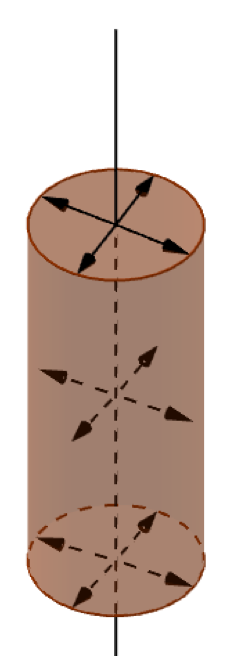
\includegraphics[height=150pt]{dlcarica}\\
	\textbf{Esempio grafico :} scelta della superficie
\end{center}
    
\pagebreak
In tale figura il contributo del campo elettrico al flusso \`e nullo per le basi del cilindro (dove le linee di campo sono parallele), mentre \`e massimo per la sua superficie laterale (in quanto ogni suo punto \`e normale alla linea di campo elettrico). Pertanto si ha che:
$$ S = S_{laterale} = 2 \pi r h $$
$$ \sum{Q_{interne}} = h\lambda $$
$$ \Phi_S\left(\vec{E}\right) = \frac{\sum{Q_{interne}}}{\varepsilon_0} = \oint_{S}{\vec{E} \cdot \hat{n}} $$
$$ \oint_{S}{\vec{E} \cdot \hat{n}} = |\vec{E}| 2\pi rh $$
$$ \frac{\cancel{h} \lambda}{\varepsilon_0} = |\vec{E}| 2\pi r \cancel{h} $$
$$ |\vec{E}| = \frac{\lambda}{2 \pi r \varepsilon_0} $$
	
$\hfill\square$
	\pagebreak
	
	    \section{Calcolare il campo elettrostatico di una distribuzione
    	piana ed uniforme di carica elettrica mediante il teorema di
    	Gauss.}
    Per distribuzione piana e uniforme di carica si intende una distribuzione di cariche su un piano nel piano $xyz$ dove vi \`e una densit\'a piana di carica $\sigma$ costante per tutto il filo.
    Si noti che :
    $$ \left[\sigma\right] =  \left[\frac{Q}{m^2}\right] $$
    
    Secondo il teorema di Gauss per il campo elettrico, vale quanto segue:
    \begin{displaymath}
    \Phi_S\left(\vec{E}\right) = \oint_{S}{\vec{E} \cdot \hat{n}} = \frac{\sum{Q_{interne}}}{\varepsilon_0}
    \end{displaymath}
    
    Per calcolare il flusso del campo elettrico su tale distribuzione occorre quindi scegliere una opportuna superfcie chiusa, per esempio un cilindro di altezza $h$ e raggio $r$ tale che intersechi il perpendicolarmente la distribuzione piana.
    
    \begin{center}
    	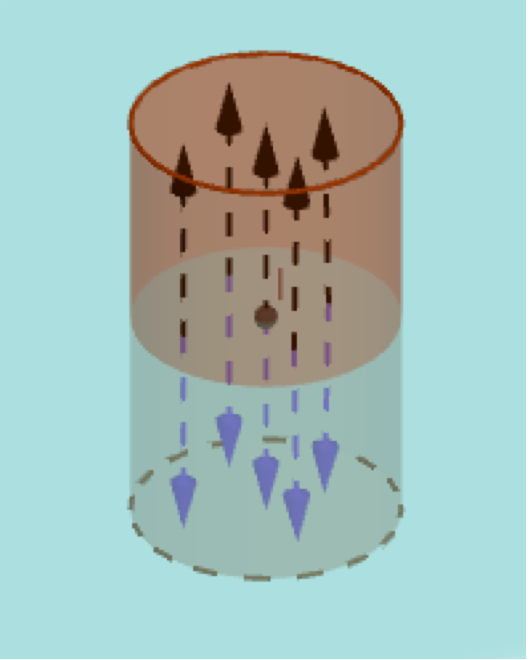
\includegraphics[height=150pt]{dpcarica}\\
    	\textbf{Esempio grafico :} scelta della superficie
    \end{center}
    
    \pagebreak
    In tale figura il contributo del campo elettrico al flusso \`e nullo per la superficie laterale del cilindro (dove le linee di campo sono parallele), mentre \`e massimo per la superficie delle basi (in quanto ogni suo punto \`e normale alla linea di campo elettrico). Pertanto si ha che:
    $$ S = 2 S_{base} = 2 \pi r^2 $$
    $$ \sum{Q_{interne}} = \sigma S_{base} $$
    $$ \Phi_S\left(\vec{E}\right) = \frac{\sum{Q_{interne}}}{\varepsilon_0} = \oint_{S}{\vec{E} \cdot \hat{n}} $$
    $$ \oint_{S}{\vec{E} \cdot \hat{n}} = 2|\vec{E}| S_{base} $$
    $$ \frac{\sigma \cancel{S_{base}}}{\varepsilon_0} = 2|\vec{E}| \cancel{S_{base}} $$
	$$ |\vec{E}| = \frac{\sigma}{2 \varepsilon_0} $$
	
	$\hfill\square$
	\pagebreak
	
	\section{Definire cos'\`e un dipolo elettrico e calcolare il campo
	elettrico sull'asse del dipolo ed il potenziale che questo
	produce.}
Un \textbf{Dipolo elettrico} \`e un sistema composto da due cariche elettriche $+q$ e $-q$ poste a una distanza $d$, costante nel tempo.

\begin{center}
	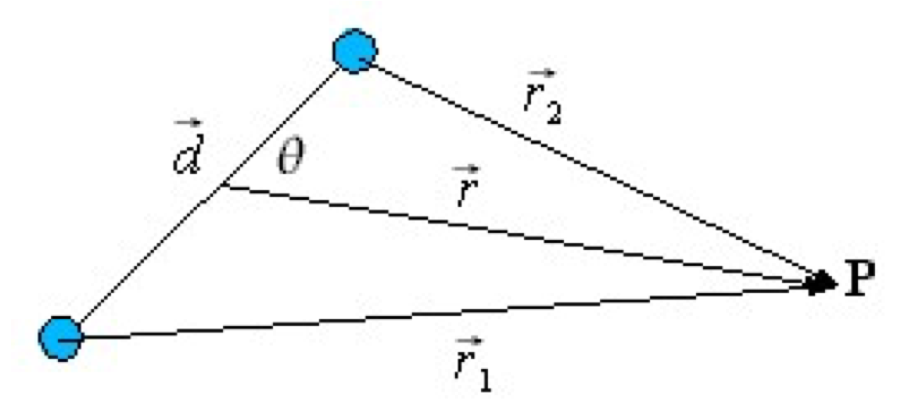
\includegraphics{dipolo} \\
	\textbf{Esempio grafico :} in un dipolo elettrico \`e interessante calcolare campo elettrico o potenziale di un dipolo in un punto generico $P$.
\end{center}

Si definisce \textbf{momento di dipolo} il seguente valore : 
\begin{equation}
    \vec{p} = q\vec{d}
\end{equation}

\textbf{Esempio 1 :} calcolo del campo elettrico lungo l'asse del dipolo.\\

Per comodit\'a si considera un dipolo di due cariche $q_1$ e $q_2$ situate nei punti A(+a, 0) e B(-a, 0), da cui ne ricaviamo il punto medio nell'origine del sistema di assi cartesiani di riferimento.\\
\\
Sapendo che il campo elettrico ha la seguente definizione
\begin{equation}
	\vec{E}(\vec{r}) = \frac{1}{4 \pi \varepsilon_0} \frac{q}{r^2} \hat{r}
\end{equation}
e per il \textbf{Principio di Sovrapposizione} sappiamo che
\begin{equation}
    \vec{E}(\vec{r}) = \sum_{j = 0}^{n_{cariche}}{\vec{E}_i(\vec{r})}
\end{equation}
Pertanto per il dipolo in questione il \textbf{Campo Elettrico} si definisce $\vec{r} = a\hat{i} + d\hat{j}$, dove $d (= 0)$ \`e la distanza del punto dall'asse del dipolo.
$$ \vec{E}(\vec{r}) = \frac{1}{4 \pi \varepsilon_0} \left(\frac{q}{(r_x - a)^2} - \frac{q}{(r_x + a)^2}\right)\hat{i} =
$$
$$ \frac{1}{4 \pi \varepsilon_0} \left(\frac{q}{(r_x - a)^2} - \frac{q}{(r_x + a)^2}\right)\hat{i} = 
$$
$$
\frac{1}{4 \pi \varepsilon_0} \left(\frac{q(r_x + a)^2 - q(r_x - a)^2}{(r_x^2 - a^2)^2}\right)\hat{i} = 
$$
$$
\frac{1}{4 \pi \varepsilon_0} \left(\frac{q\left[(r_x + a)^2 - (r_x - a)^2\right]}{(r_x^2 - a^2)^2}\right)\hat{i}
$$
Usando il metodo della \textbf{differenza dei quadrati} $\left[a^2 - b^2 = (a+b)(a-b)\right]$:
$$
\frac{1}{4 \pi \varepsilon_0} \left(\frac{q\left[(2r_x)(2a)\right]}{(r_x^2 - a^2)^2}\right)\hat{i} = 
$$
$$
\frac{1}{4 \pi \varepsilon_0} \left(\frac{4qar_x}{(r_x^2 - a^2)^2}\right)\hat{i}
$$
imponendo $2a = d$ (poich\`e $+a$ e $-a$ rappresentano dove si trovano le cariche sull'asse e la loro distanza \`e appunto $2a$):
$$
\frac{1}{4 \pi \varepsilon_0} \left(\frac{2qdr_x}{\left[r_x^2 - \left(\frac{d}{2}\right)^2\right]^2}\right)\hat{i}
$$
in termini del \textbf{momento di dipolo} dato da (8):
$$
\frac{1}{4 \pi \varepsilon_0} \left(\frac{2pr_x}{\left[r_x^2 - \left(\frac{d}{2}\right)^2\right]^2}\right)\hat{i}
$$
Ipotizzando che $r_x >> d$ si ottiene:
$$
\frac{ 1 }{ 4 \pi \varepsilon_0 } 
\frac{ 2pr_x }{ (r_x^2)^2 } 
\hat{ i } = 
\frac{ 1 }{ 4 \pi \varepsilon_0 } 
\frac{ 2p\cancel{ r_x } }{ r_x^{\cancel{ 4 }^3} } 
\hat{ i } = 
\frac{ 1 }{ 4 \pi \varepsilon_0 } 
\frac{ 2p}{ r_x^3 } 
\hat{ i }
$$
$\hfill\square$ \\
\textbf{Esempio 2 :} Calcolo del \textbf{potenziale elettrico} del dipolo sull'asse del dipolo.\\
Si ricorda la formula del potenziale elettrico come:
$$
  V(r_x) = \frac{1}{4 \pi \varepsilon_0}\frac{q}{r}
$$ 
Anche qui vale il \textbf{Principio di Sovrapposizione}:
$$
  V(r) = \sum_{k = 0}^{n_{cariche}}{V_i(r)}
$$
Si fanno le stesse premesse dell'esempio 1.\\
$$ V(r_x) = \frac{1}{4 \pi \varepsilon_0} \left(\frac{q}{r_x - a} - \frac{q}{r_x + a}\right) =
$$
$$
\frac{1}{4 \pi \varepsilon_0} \left(\frac{q(r_x + a) - q(r_x - a)}{r_x^2 - a^2}\right) = 
$$
$$
\frac{ 1 }{ 4 \pi \varepsilon_0 } \left( \frac{ q \left[ \cancel{ r_x } + a - \cancel{ r_x } + a \right] }{ r_x^2 - a^2 } \right) =
$$
$$
\frac{1}{4 \pi \varepsilon_0} \left(\frac{2aq}{r_x^2 - a^2}\right) =
$$
imponendo $2a = d$
$$
\frac{ 1 }{ 4 \pi \varepsilon_0 } 
\left( 
    \frac{ dq }{ r_x^2 - 
	\left( 
        \frac{ d }{ 2 } 
    \right) ^2 
    } 
\right) =
$$
in termini del \textbf{momento di dipolo} dato da (8):
$$
\frac{1}{4 \pi \varepsilon_0} \left(\frac{p}{r_x^2 - \left(\frac{d}{2}\right)^2}\right)
$$
Ipotizzando che $r_x >> d$ si ottiene:
$$
\frac{1}{4 \pi \varepsilon_0} \left(\frac{p}{r_x^2}\right) = \frac{ p }{ 4 \pi \varepsilon_0 r_x^2}
$$
$\hfill\square$ \\
	\pagebreak
	
	\section{Dimostrare che la forza di Coulomb è una forza
	conservativa e discutere brevemente le conseguenze di
	questo.}
Si dice che una forza \`e conservativa quando:
$$
   L_{\vec{r}_a \rightarrow \vec{r}_b} = U(B) - U(A)
$$
Si definisce il lavoro come :
$$
   L_{\vec{r}_a \rightarrow \vec{r}_b} = 
   \int_A^B{\vec{F_{\vec{r}_a \rightarrow \vec{r}_b}} \cdot \vec{ds}}
$$
Un'esempio di forza non conservativa \`e l'attrito.
Per quanto riguarda la forza di Coulomb invece si puo' affermare che:
\begin{displaymath}
    L_{\vec{r}_a \rightarrow \vec{r}_b} =
    \int_A^B{\vec{F_{\vec{r}_a \rightarrow \vec{r}_b}} \cdot \vec{ds}} =
    \int_A^B{ 
    	\frac{ 1 } { 4 \pi \varepsilon_0 } 
    	\frac{ q_1 q_2 }{ (r_b - r_a)^2 } 
        \hat{u}_{r_a \rightarrow r_b} \cdot \vec{ ds }
        }
\end{displaymath}
Definiamo $\vec{r} = \vec{r}_b - \vec{r}_a$ e riscriviamo come
\begin{displaymath}
    \int_A^B{ 
    	\frac{ 1 } { 4 \pi \varepsilon_0 } 
    	\frac{ q_1 q_2 }{ r^2 } 
    	\hat{u}_r \cdot \vec{ ds }
    } = 
    \int_A^B{ 
    	\frac{ 1 } { 4 \pi \varepsilon_0 } 
    	\frac{ q_1 q_2 }{ r^2 } 
    	\vec{dr}
    } =  
  	\frac{ 1 } { 4 \pi \varepsilon_0 } 
    \int_A^B{ 
    	\frac{ q_1 q_2 }{ r^2 } 
    	\vec{dr}
    }
\end{displaymath}
\begin{displaymath}
\frac{ 1 }{ 4 \pi \varepsilon_0 }
\left[ 
-\frac{ q_1 q_2 }{r}
\right]_A^B = 
\frac{ 1 }{ 4 \pi \varepsilon_0 }
\left(
    \frac{ q_1 q_2 }{r_A} - \frac{ q_1 q_2 }{r_B}
\right) = 
U(r_A) - U(r_B)
\end{displaymath}
Come conseguenza di questo si puo' affermare che il \textbf{Lavoro} compiuto dalla forza di Coulomb su un percorso chiuso \`e nullo:
$$
    L_{A \rightarrow B} + L_{B \rightarrow A} = 0
$$
Si puo' inoltre affermare che il Lavoro compiuto dalla Forza di Coulomb non dipende dal percorso fra A e B.
$\hfill\square$
	\pagebreak
	
	\section{Definire potenziale, energia potenziale e lavoro del
	campo elettrico e mostrare le relazioni tra queste
	grandezze.}
Per \textbf{Energia Potenziale Elettrica} di un sistema di cariche si intende il lavoro compiuto da tale sistema per potersi spostare da una configurazione all'infinito (dove per convenzione l'energia potenziale \`e nulla) da una configurazione data.
Nel caso di due cariche puntiformi $q_1$ e $q_2$, in cui :
$$
   U_{q_1}(r) = 0 
$$
poich\'e \`e inserita per prima nel sistema
$$
   U_{q_1, q_2}(r) = \frac{1}{4 \pi \varepsilon_0} \frac{q_1 q_2}{r}
$$
poich\'e ora \`e soggetta a una forza fra $q_1$ e $q_2$.\\
\\
Il lavoro necessario a tale forza per muovere le cariche da una configurazione A a infinito  \`e:
$$
L_{A \rightarrow \infty} = 
\int_A^{\infty}{\vec{F} \cdot \vec{ds}} = 
\int_A^{\infty}{
	\frac{1}{4 \pi \varepsilon_0} \frac{q_1 q_2}{r^2}\hat{u}_r \cdot \vec{ds}
} =
$$
$$
  \int_A^{\infty}{
  	\frac{1}{4 \pi \varepsilon_0} \frac{q_1 q_2}{r^2}\vec{dr}
  } = 
  \frac{q_1 q_2}{4 \pi \varepsilon_0}
  \left[
      -\frac{1}{r}
  \right]_A^{\infty} = 
  \frac{q_1 q_2}{4 \pi \varepsilon_0} 
  \left(
     \frac{1}{r_A} - 0
  \right) =
$$
$$
  \frac{1}{4 \pi \varepsilon_0} \frac{q_1 q_2}{r_A}
$$
Per \textbf{Potenziale Elettrico} di una carica $Q$ si intende l'energia potenziale U di un sistema composto da $Q$ e una carica di prova $q_{test}$, cio\'e come :
$$
  V(r) = \frac{U}{q_{test}} = 
  \frac{1}{4 \pi \varepsilon_0}
  \frac{Q \cancel{q_{test}}}{r}
  \frac{1}{\cancel{q_{test}}} =
  \frac{1}{4 \pi \varepsilon_0} \frac{Q}{r}
$$
Per \textbf{Lavoro} del campo elettrico si intende il lavoro necessario per spostare una carica $q$ immersa in un campo elettrico $ \vec{E} $ dovuto a una carica $Q$ da un punto $A$ a un punto $B$ e corrisponde a :
$$ 
     L_{r_A \rightarrow r_B} = \int_{A}^{B}{q \vec{E} \cdot  \vec{ds}} =  
     \frac{1}{4 \pi \varepsilon_0}\int_{A}^{B}{q \frac{Q}{r^2} \hat{r} \cdot \vec{ds}} = \frac{qQ}{4 \pi \varepsilon_0} \int_{A}^{B}{\frac{1}{r^2} \hat{r} \cdot \vec{ds}} =
$$
$$
    \frac{qQ}{4 \pi \varepsilon_0} \int_{A}^{B}{\frac{1}{r^2} \vec{dr}} = \frac{qQ}{4 \pi \varepsilon_0} \left[-\frac{1}{r}\right]_A^B = \frac{qQ}{4 \pi \varepsilon_0} \left(-\frac{1}{r_B} + \frac{1}{r_A} \right) = 
$$
$$
    \frac{qQ}{4 \pi \varepsilon_0 r_A} - \frac{qQ}{4 \pi \varepsilon_0 r_B} = U(r_A) - U(r_B)
$$
$\hfill\square$
	\pagebreak
	
	\section{Condensatore piano: calcolare l'andamento del campo
	elettrico, e del potenziale dentro e fuori il condensatore e la
	sua capacità.}
Il condensatore piano \`e un sistema costituito da due superfici $piane$ di materiale conduttore, di superficie $S$, posti a una distanza $d$ e in modo da costituire due piani paralleli. Inoltre una superficie \`e caricata positivamente e l'altra negativamente.\\
\begin{center}
	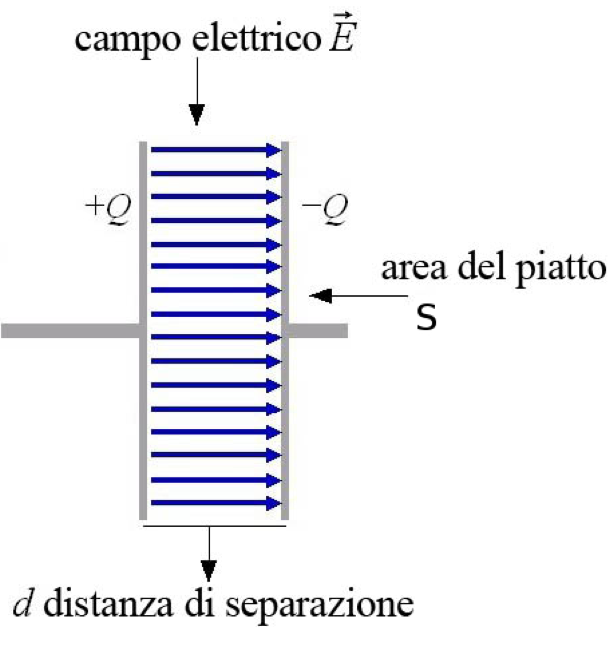
\includegraphics[height=5cm]{condensatore_piano}
\end{center}
\textbf{Esempio grafico :} come si puo' notare, all'interno di un condensatore piano vi \`e un campo elettrico uniforme.\\
Si definisce come \textbf{Capacit\'a} di un condensatore la quantit\'a di carica immagazzinabile sulle armature per unit\'a di differenza di potenziale ai capi delle armature.\\
$$
    C = \frac{Q}{\Delta V}
$$
All'esterno del condensatore il campo elettrico \`e nullo, poich\'e esso \`e isolato. $\left(\vec{E} = 0\right)$
Per calcolare il campo elettrico all'interno sfruttiamo il \textbf{Teorema di Gauss per il campo elettrico}: \\
\`E il caso della distribuzione piana di carica, assumiamo $\sigma$ come densita piana di carica:
$$
   \left[\sigma\right] = \left[\frac{Q}{L^2}\right]
$$
Intersechiamo un cilindro di raggio $r$ e lunghezza $l$ con un piano del condensatore, in modo tale che esso abbia entrambe le basi parallele al piano.

\pagebreak

Grazie a cio' possiamo affermare che il contributo al flusso delle basi \`e nullo, mentre \`e massimizzato sulla superficie laterale(dove le linee di campo sono perpendicolari).\\
$$
    \Phi(\vec{E}) = \frac{\sum{Q_{interne}}}{\varepsilon_0} = \oint_S{\vec{E} \cdot \hat{n}}
$$
Formalizziamo la affermazione precedente:
$$
    S = 2 S_{base} = \pi r^2
$$
inoltre si ha che
$$
    \sum{Q_{interne}} = \sigma S_{base}
$$
e calcoliamo il campo elettrico:
$$
    \frac{\sum{Q_{interne}}}{\varepsilon_0} = \oint_S{\vec{E} \cdot \hat{n}}
$$
$$
    \frac{\sigma S_{base}}{\varepsilon_0} = \oint_S{E}
$$
$$
    \frac{\sigma \cancel{S}}{\varepsilon_0} = 2 E \cancel{S}
$$
$$
    E = \frac{\sigma}{2 \varepsilon_0}
$$
Si noti che il capo elettrico in realt\'a \`e per una sola delle armature, pertanto 
$$
    E_{totale} = 2 E = \cancel{2} \frac{\sigma}{\cancel{2} \varepsilon_0} = \frac{\sigma}{\varepsilon_0}
$$
Per il calcolo della Capacit\'a bisogna calcolare la differenza di potenziale $\Delta V$ come :
$$
    \Delta V = \int_{A}^{B}{\vec{E} \cdot \vec{ds}} = \frac{\sigma}{\varepsilon_0}d
$$
Dove $d$ \`e la distanza fra le armature.\\
Pertanto:
$$
    C = \frac{Q}{\Delta V} = Q \frac{\varepsilon_0}{\sigma d} = 
    \cancel{\sigma} S \frac{\varepsilon_0}{\cancel{\sigma} d} = \frac{S\varepsilon_0}{d}
$$
$\hfill\square$
	\pagebreak
	
	\section{Spiegazione del comportamento di resistori in serie ed in
	parallelo. Determinazione della resistenza equivalente.}

Si definisce \textbf{Resistenza Equivalente} di una rete di resistori la resistenza di un singolo resistore che, sottoposto alla stessa differenza di potenziale $\Delta V$ a cui \`e soggetta la rete, assorbe la stessa corrente elettrica.

Nel caso di resistori in serie avviene che:\\
\\
\noindent\begin{minipage}{0.3\textwidth}
$
\left\{
\begin{array}{lr}
	V_A - V_B = i R_1 \\	
	V_B - V_C = i R_2	\\	
	V_A - V_C = i R_{eq} \\
	V_A - V_B + V_B - V_C = V_A - V_C \\
	\\
	\textnormal{Passaggi Algebrici:}\\
	\cancel{i} R_1 + \cancel{i} R_2 = \cancel{i} R_{eq} \\
	R_1 + R_2 = R_{eq}
\end{array}
\right.
$
\end{minipage}
\hfill%
\begin{minipage}{0.6\textwidth}\raggedleft
	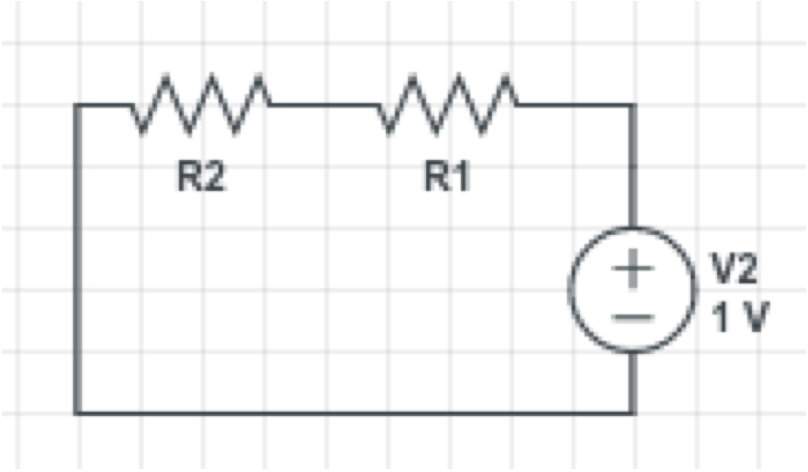
\includegraphics{serie_res}
\end{minipage}
Pertanto la $R_{eq}$ vale $R_1 + R_2$.\\
Nel caso di $n$ resistori vale la seguente formula:
\begin{equation}
    R_{eq} = \sum{R_i}
\end{equation}
Dove tutte le $R_i$ sono in serie sullo stesso ramo.\\
\noindent\begin{minipage}{0.3\textwidth}
	$
	\left\{
	\begin{array}{lr}
	V_A - V_B = i_1 R_1 \\	
	V_A - V_B = i_2 R_2	\\	
	V_A - V_B = i R_{eq} \\
	i = i_1 + i_2 \\
	\\
	\textnormal{Passaggi Algebrici:}\\
	R_{eq} = \frac{V_A - V_B}{i_1 + i_2}\\
	\frac{\cancel{V_A - V_B}}{\frac{\cancel{V_A - V_B}}{R_1} + \frac{\cancel{V_A - V_B}}{R_2}} = R_{eq}\\	
	\frac{1}{\frac{1}{R_1} + \frac{1}{R_2}} = R_{eq}\\	
	\frac{1}{R_eq} = \frac{1}{R_1} + \frac{1}{R_2}
	\end{array}
	\right.
	$
\end{minipage}
\hfill%
\begin{minipage}{0.6\textwidth}\raggedleft
	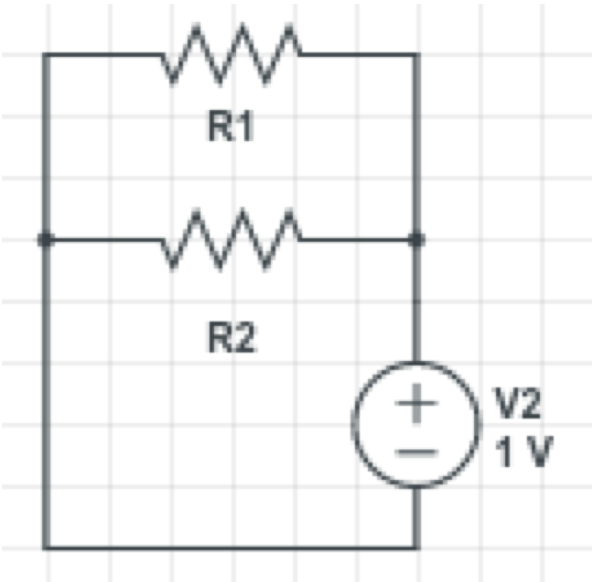
\includegraphics{parall_res}
\end{minipage}
Pertanto la $R_{eq}$ vale $\frac{1}{R_1} + \frac{1}{R_2} = \frac{R_1 + R_2}{R_1 R_2}$.\\
Nel caso di $n$ resistori vale la seguente formula:
\begin{equation}
    R_{eq} = \sum{\frac{1}{R_i}}
\end{equation}
Dove tutte le $R_i$ sono in  sullo stesso ramo.
$\hfill\square$
	\pagebreak
	
	\section{Spiegazione del comportamento di condensatori in
	serie ed in parallelo. Determinazione della capacit\'a
	equivalente.}

Si definisce \textbf{Capacit\'a Equivalente} di una rete di condensatori la capacit\'a di un singolo condensatore che, sottoposto alla stessa differenza di potenziale $\Delta V$ a cui \`e soggetta la rete, assorbe la stessa corrente elettrica.

Nel caso di condensatori in serie avviene che, essendoci su tutto il ramo la stessa quantit\'a di carica :\\
\\
\noindent\begin{minipage}{0.3\textwidth}
$
\left\{
\begin{array}{llr}
	V_A - V_B = \frac{1}{C_1}Q_1 \\
	V_B - V_C = \frac{1}{C_2}Q_2 \\	
	V_A - V_C = \frac{1}{C_{eq}}Q_{eq} \\
	V_A - V_B + V_B - V_C = V_A - V_C  \\
	Q_1 = Q_2 = Q_{eq} = Q \\
	\\
	\textnormal{Passaggi Algebrici:}\\
	\frac{1}{C_1}\cancel{Q} + \frac{1}{C_2}\cancel{Q} = \frac{1}{C_{eq}}\cancel{Q} \\
	\frac{1}{C_1} + \frac{1}{C_2} = \frac{1}{C_{eq}}
\end{array}
\right.
$
\end{minipage}
\hfill%
\begin{minipage}{0.6\textwidth}\raggedleft
	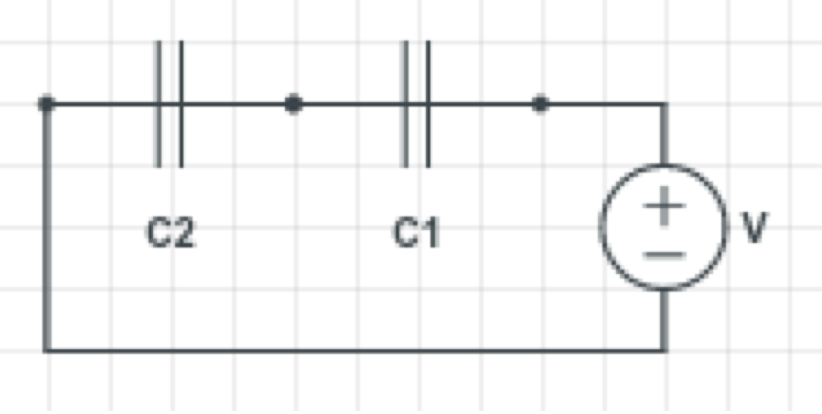
\includegraphics{serie_cond}
\end{minipage}
Pertanto la $C_{eq}$ vale $\frac{1}{C_1} + \frac{1}{C_2}$.\\
Nel caso di $n$ condensatori vale la seguente formula:
\begin{equation}
    C_{eq} = \sum{\frac{1}{C_i}}
\end{equation}
Dove tutte le $C_i$ sono in serie sullo stesso ramo.\\
\noindent\begin{minipage}{0.3\textwidth}
	$
	\left\{
	\begin{array}{lr}
	V_A - V_B = \frac{Q_1}{C_1} \rightarrow C_1 = \frac{Q_1}{V_A - V_B}   \\
	V_A - V_B = \frac{Q_2}{C_2}	\rightarrow C_2 = \frac{Q_2}{V_A - V_B}   \\
	V_A - V_B = \frac{Q_{eq}}{C_{eq}} \\
	Q_{eq} = Q_1 + Q_2\\
	\\
	\textnormal{Passaggi Algebrici:}\\
	V_A - V_B = \frac{Q_{eq}}{C_{eq}} = \frac{Q_1 + Q_2}{C_{eq}} = \\
	\frac{C_1(V_A - V_B) + C_2(V_A - V_B)}{C_{eq}} = \\
	\frac{(V_A - V_B)(C_1 + C_2)}{C_{eq}} \rightarrow \cancel{(V_A - V_B)} = \frac{\cancel{(V_A - V_B)}(C_1 + C_2)}{C_{eq}} \\
	C_{eq} = C_1 + C_2
	\end{array}
	\right.
	$
\end{minipage}
\hfill%
\begin{minipage}{0.6\textwidth}\raggedleft
	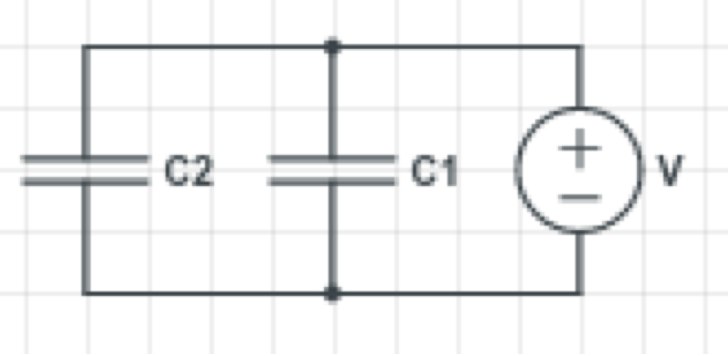
\includegraphics{parall_cond}
\end{minipage}
Pertanto la $C_{eq}$ vale $C_1 + C_2$.\\
Nel caso di $n$ resistori vale la seguente formula:
\begin{equation}
    R_{eq} = \sum{C_i}
\end{equation}
Dove tutte le $C_i$ sono in parallelo sullo stesso ramo.\\
\textbf{[Opzionale, dimostrare (11), (12), (13) e (14) per induzione su n]}
\begin{flushright}
	$\square$
\end{flushright}
	\pagebreak
	
	\section{Circuiti RC: carica e scarica del condensatore.
	Comportamento alla stazionarietà.}
Per \textbf{Processo di carica} del condensatore si intende l'accumulo di carica sulle armature dello stesso quando \`e applicata una differenza di potenziale $\Delta V$.\\
Allo stesso modo si definisce \textbf{Processo di scarica} del condensatore il rilascio delle cariche precedentemente accumulate, facendo generare allo stesso una differenza di potenziale.\\
\textbf{Fase di carica} :\\
Vale la seguente legge:
$$
    Q(t) = Q_{MAX}\left(1 - e^{-\frac{t}{RC}}\right)
$$
$$
    Q(t) = C \Delta V\left(1 - e^{-\frac{t}{RC}}\right)	 
$$
\begin{itemize}
	\item [$t < 0$] { Condensatore scarico, $\Delta V = 0$ }
	\item [$t \rightarrow 0$] { 
		Condensatore in carica, $\Delta V = \varepsilon$ 
		carica il condensatore : \\
	        $$
	           Q(t) = Q_{MAX}\left(1 - e^{-\frac{0}{RC}}\right) = Q\left(1 - 1\right) = 0
	        $$
    }
    \item [$t \rightarrow \infty$] { 
    	Condensatore carico a regime,
    	$\Delta V(t)$ carica il condensatore:
    	$$
    	    Q(t) = Q_{MAX}\left(1 - e^{-\frac{\infty}{RC}}\right) = 
    	    Q_{MAX}\left(1 - e^{-\infty}\right) = 
    	    Q_{MAX}\left(1 - 0\right) = Q_{MAX} = C \varepsilon
    	$$
    }
\end{itemize}
\textbf{ Fase di scarica } :
Vale la seguente legge :
$$
    Q(t) = C \Delta V \left(e^{-\frac{t}{RC}}\right)
$$
\begin{itemize}
	\item [$t < 0$] {
		Il condensatore \`e carico. 
		$\Delta V = \varepsilon$, 
		$Q(t) = Q_{MAX} = C \varepsilon$ 
	}
	\item [$t \rightarrow 0$] {
        Il condensatore inizia a scaricarsi.\\
        $\Delta V = 0$, $Q(t) = Q_{MAX}\left(e^{-\frac{0}{RC}}\right) = 
        Q_{MAX}\left(e^0\right) = C \varepsilon$\\
        Si comporta come un \textbf{generatore di corrente} :
        $$
        \varepsilon_C = \frac{Q_C}{C}
        $$
	}
	\item [$t \rightarrow \infty$] { 
	    Il condensatore \`e scarico.\\
	    $\Delta V = 0$, 
    	$
    	Q(t) = Q_{MAX}\left(e^{-\frac{\infty}{RC}}\right) = 
    	Q_{MAX}\left(e^{-\infty}\right) = Q_{MAX} \cdot 0 = 0
    	$ 
	}
\end{itemize}
$\hfill\square$
	\pagebreak
	
	\section{Leggi di Ohm microscopica e derivazione della legge
	macroscopica a partire da quella microscopica.}
Si definisce \textbf{Intensit\'a di corrente} la quantit\'a di carica che passa in un conduttore per unit\'a di tempo.
$$ [I] = \left[\frac{Q}{t}\right] $$
Per dare una definizione microscopica della legge di Ohm occorre considerare gli elettroni che si muovono all'interno di conduttore di sezione $S$. Applicando ai suoi estremi una differenza di potenziale si crea un campo elettrico, che fa muovere gli elettroni di una velocit\'a $v_d$ (velocit\'a di deriva) in modo collettivo e ordinato, oltre che del canonico moto casuale dovuto alla instabilit\'a dell'elettrone stesso.\\
Ora la nuova definizione di intensit\'a di corrente \`e la seguente:
$$
I = n e v_d S
$$
Dove:
\begin{itemize}
	\item [n] {Il numero di elettroni che passano per unita di volume}
	\item [e] {La carica dell'elettrone}
	\item [$v_d$] {La velocit\'a di deriva}
	\item [S] {La sezione del conduttore}
\end{itemize}
Ora si introduce la grandezza \textit{conduttivit\'a elettrica} indicata con $\sigma$ e il vettore $\vec{J} = \sigma \vec{E}$ "densit\'a di corrente".\\
$$
    \sigma = n e v_d
$$
$$
    \rho = \frac{1}{\sigma}
$$
La densit\'a di corrente rappresenta la "facilit\'a" con cui gli elettroni si muovono all'interno del campo elettrico nel conduttore.
Consideriamo un tratto di lunghezza $l$ del conduttore: allora si puo' affermare che (assumendo il campo elettrico ORTOGONALE alla sezione del conduttore):
$$
    I = \int{\vec{J} \cdot \vec{dS}} = \int{\sigma E \cdot \vec{dS}} = \sigma E S
$$
Considerando il campo elettrico uniforme, abbiamo che $E = \frac{V}{l}$, pertanto:
$$
    I = \sigma \frac{V}{l}S \rightarrow V = \frac{l}{\sigma S} \rightarrow V = RI
$$
$\hfill\square$
	\pagebreak
	
	\section{Descrivere le equazioni del moto di una carica elettrica
	in un campo magnetico uniforme.}
Una carica elettrica immersa in un campo magnetico \`e soggetta a una forza (chiamata \textbf{Forza di Lorentz}) cosi definita:
$$
    \vec{F} =  q\vec{v} \times \vec{B}
$$
Dove:
\begin{itemize}
	\item [$q$] { La carica elettrica. }
	\item [$\vec{v}$] { La velocit\'a del moto della carica. }
	\item [$\vec{B}$] { Il campo magnetico in cui la carica \`e immersa. }
\end{itemize}
A seconda dei casi il contributo \`e differente :
\begin{itemize}
	\item [caso $\vec{v} \parallel \vec{B}$] { Il prodotto vettoriale \`e nullo, pertanto la particella non \`e soggetta a forza magnetica. }
	\item [caso $\vec{v} \perp \vec{B}$] { Il prodotto vettoriale \`e massimizzato e di direzione perpendicolare al piano contenente $\vec{v}$ e $\vec{B}$. Per il verso si usa la regola della mano destra.
		Nel caso $B$ sia costante si ha un moto su traiettoria circolare. }
	\item [caso : moto a elica] { 
		Si scompone il vettore $\vec{v}$ in 2 componenti perpendicolari fra loro : \\
		$\vec{v} = \vec{v}_{\parallel} + \vec{v}_{\perp}$ dove:
		\begin{itemize}
			\item [$\bullet$] { 
				$\vec{v}_{\parallel}$ non da alcun contributo alla forza.
			}
			\item [$\bullet$] { $\vec{v}_{\perp}$ produce una forza ortogonale al piano contenente $\vec{v}$ e $\vec{B}$. }
		\end{itemize}
		La combinazione dei due moti genera un moto elicoidale avente asse coincidente con $\hat{u}_B$ 
	}
\end{itemize}
$\hfill\square$
	\pagebreak
	
	\section{Determinare la forza tra due fili paralleli percorsi da
	correnti stazionarie e discutere la relazione con la terza
	legge di Newton.}
Un filo rettilineo percorso da una corrente $I$ produce a una distanza $r$ una campo magnetico, il cui modulo \`e dato dalla seguente formula:
\begin{equation}
 	B = \mu_0 \frac{I}{2 \pi r}
\end{equation}
Le cui linee di forza sono circonferenze aventi centro \textbf{sull'asse del filo stesso} (Il verso \`e determinato dal \textbf{verso della corrente}, attraverso la regola della mano destra).\\
Se si fanno interagire due fili paralleli, accade che vi \`e una mutua interazione: 

\noindent\begin{minipage}{0.4\textwidth}
	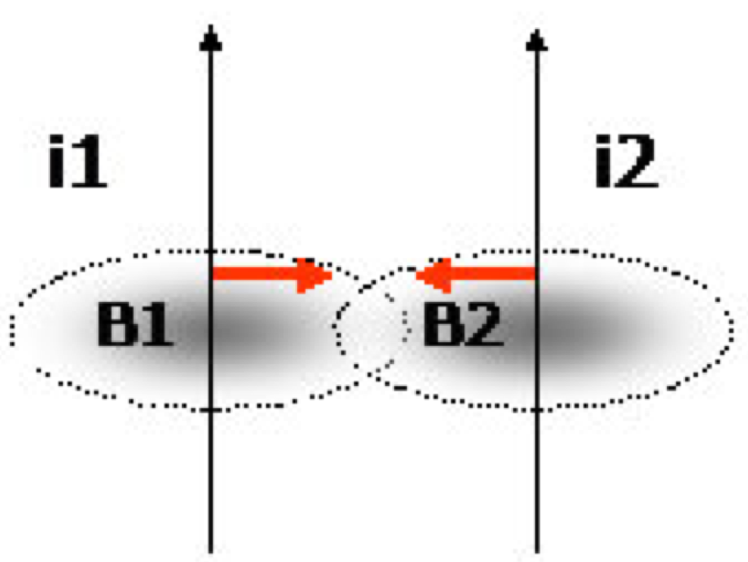
\includegraphics[width=5cm]{fili_1}
\end{minipage}
\hfill%
\begin{minipage}{0.4\textwidth}\raggedleft
	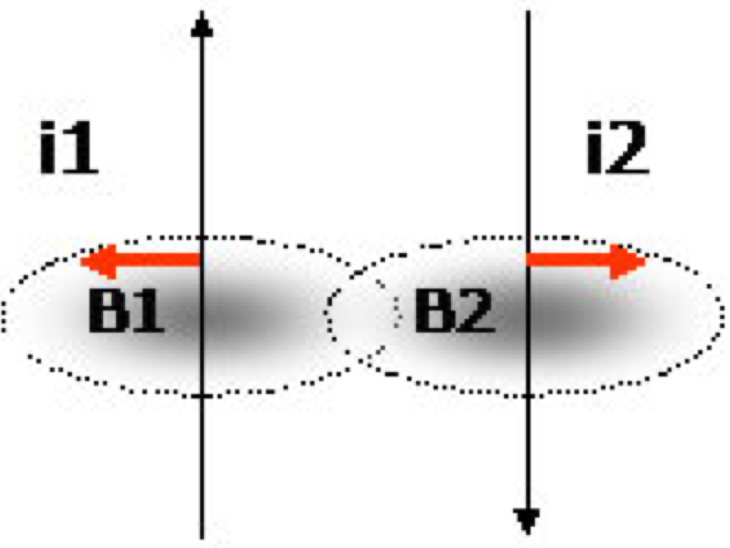
\includegraphics[width=5cm]{fili_2}
\end{minipage}\\
 Sul filo 1 vi \`e una forza dovuta al campo $B_2$ mentre sul filo 2 vi \`e una forza dovuta a $B_1$. Si ha pertanto che:
 $$
     F_{1 \rightarrow 2} = B_2 I_1 d = \mu_0 \frac{I_2}{2 \pi d}I_1 = \mu_0 \frac{I_1 I_2}{2 \pi d}l
 $$
 $$
     F_{2 \rightarrow 1} = B_1 I_2 d = \mu_0 \frac{I_1}{2 \pi d}I_2 = \mu_0 \frac{I_1 I_2}{2 \pi d}l
 $$
 Dove $d$ \`e la distanza fra i due fili e $l$ \`e la lunghezza del tratto di filo considerato.\\
 La forza \`e attrattiva se i versi delle correnti sono \textbf{concordi}, mentre \`e repulsiva se sono \textbf{discordi}.
 Si noti che, proprio come in base alla Terza Legge di Newton, si ha che :
 $$
     \vec{F}_{1 \rightarrow 2} = -\vec{F}_{2 \rightarrow 1}
 $$
 $\hfill\square$

	\pagebreak
	
	\section{Enunciare la legge di Bi\^ot-Sav\`art ed usarla per il
	calcolo del campo magnetico prodotto da una spira circolare
	percorsa da corrente stazionaria sull'asse della spira.}
Secondo la \textbf{Legge di Bi\^ot-Sav\`art} vale che :
$$
    d\vec{B} = \frac{\mu_0}{4 \pi} i \frac{d\vec{l} \times \hat{r}}{r^2}
$$
Dove : 
\begin{itemize}
	\item [$i$] {
	    Intensit\'a di corrente che scorre nella \textbf{spira circolare}.	
	}
	\item[$d\vec{l}$] {
	    Tratto di lunghezza \textbf{infinitesima} del filo della spira.
	}
	\item[$\vec{r}$] {
	    Raggio-vettore che individua il punto $P$ nel quale si vuole misurare il campo $d\vec{B}$.	
	}
\end{itemize}
INCOMPLETA!!!!
	\pagebreak
	
	\section{Enunciare la legge di Amp\'ere ed usarla per il calcolo
	del campo magnetico all'interno di un solenoide rettilineo
	percorso da corrente stazionaria.}
Secondo la \textbf{Legge di Amp\'ere}:
$$
    \Gamma_B = \mu_0 I_{conc}
$$
Dove :
\begin{itemize}
	\item [$\Gamma_B$] {
		\`e la circuitazione del campo magnetico $B$ sulla    linea chiusa $l$, ovvero :
        $$
            \Gamma_B = \oint_l{\vec{B}} = \oint{\vec{B} \cdot d\vec{l}}
        $$
    }
    \item [$I_{conc}$] {
    	\`e la somma delle correnti concatenate al percorso \textbf{chiuso} su cui si esegue la circuitazione.
    }
\end{itemize}
\begin{center}
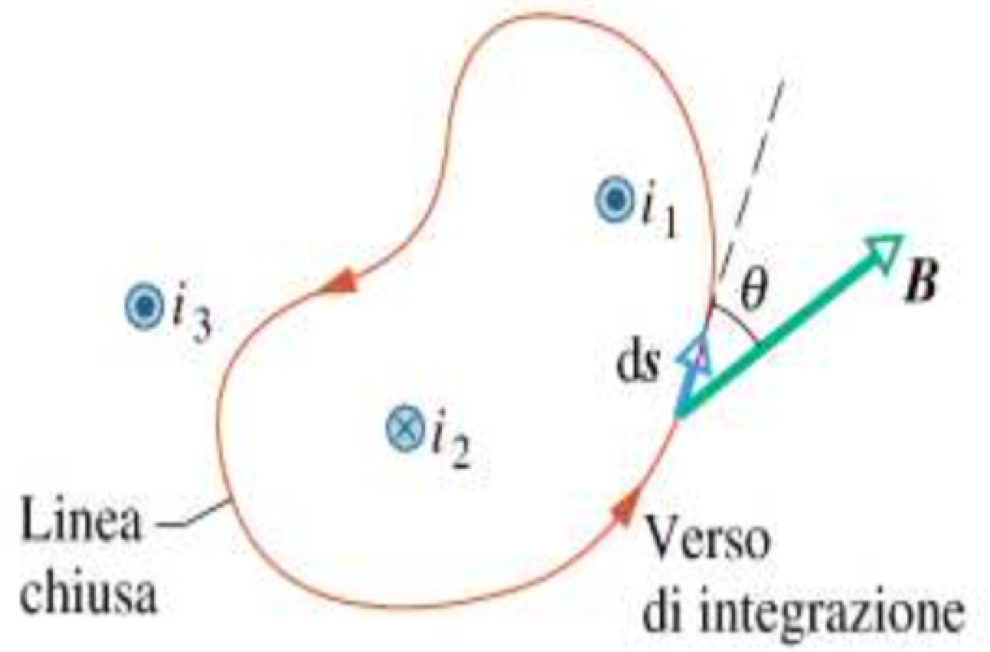
\includegraphics[width=0.6\textwidth]{ampere_1}
\end{center}

\pagebreak

Un esempio di applicazione consiste nel considerare un solenoide lungo $l$ avente $n$ spire per unit\'a di lunghezza. \\
Esso \`e percorso da un campo magnetico $\vec{B}$ uniforme, dove le sue linee sono orientate parallelamente all'asse. Scegliamo la circuitazione come un quadrato di lato $h$ lungo i punti $a$, $b$, $c$, $d$ come da immagine.
\begin{center}
	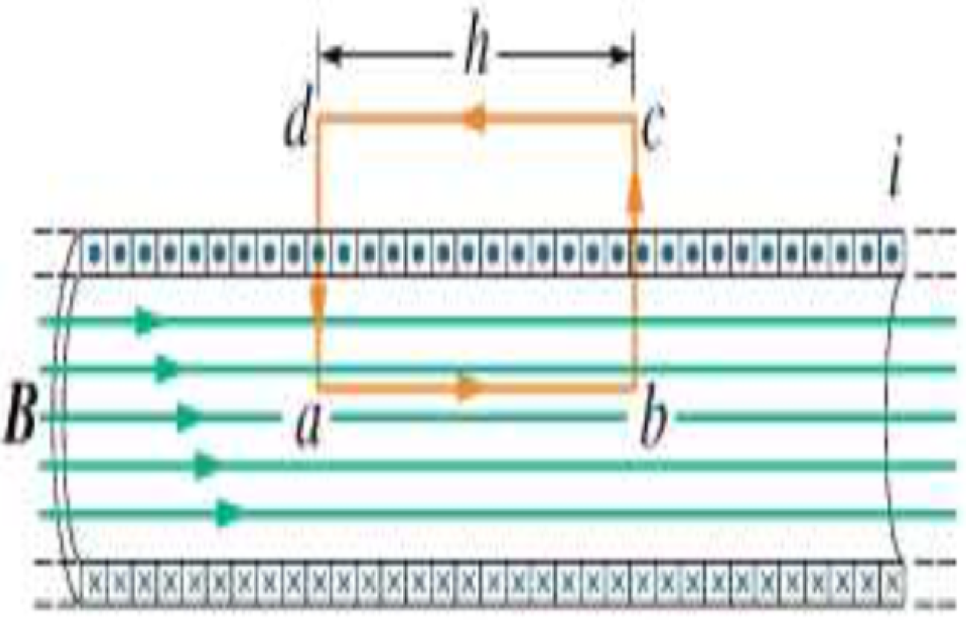
\includegraphics[width=0.6\textwidth]{ampere_2}
\end{center}
Abbiamo quindi che:
$$
     \Gamma_B = \oint_{abcd}{\vec{B}} = \oint_{ab}{\vec{B}} + \oint_{bc}{\vec{B}} + \oint_{cd}{\vec{B}} + \oint_{da}{\vec{B}}
$$
Da cui assumiamo che : 
\begin{itemize}
	\item [$\oint_{cd}{\vec{B}} = 0$] {
	    Poich\'e $cd$ non \`e all'interno del solenoide.	
	}
	\item [$\oint_{bc}{\vec{B}} = \oint_{da}{\vec{B}} = 0$] {
		Poich\'e $\vec{bc} \perp \vec{B} \land da \perp \vec{B} \land \vec{V_1} \perp \vec{V_2} \Longrightarrow \vec{V_1} \cdot \vec{V_2} = 0$
	}
	\item [$\oint_{ab}{\vec{B}}$] {
		Siccome $\vec{ab} \parallel \vec{B}$ vale che:
		$$
	        \oint_{ab}{\vec{B}} = \int{\vec{B} \cdot d\vec{ab}} = Bh
		$$
	}
\end{itemize}
Sfruttando questo eguagliamo:
$$
    \Gamma_B = \oint_{abcd}{\vec{B}} = \oint_{ab}{\vec{B}} = Bh
$$
$$
    Bh = \mu_0 I_{conc}
$$
Da cui si conclude che :
$$
    B = \mu_0 \frac{I_{conc}}{h} = \mu_0 \frac{n \cancel{h} i}{\cancel{h}} = \mu_0 n i
$$
Dove : 
\begin{itemize}
	\item [n] {\`e il numero di spire per unit\'a di lunghezza }
	\item [i] {\`e la corrente che scorre nel solenoide}
\end{itemize}
Si noti che : $I_{conc} = n h i$.
$\hfill\square$
	\pagebreak
	
	\section{Enunciare la legge di Faraday-Lenz e discutere la
	relazione con l'autoinduttanza.}
Secondo la \textbf{Legge di Faraday-Lenz} :
\begin{equation}
	\varepsilon_{indotta} = -\frac{d\Phi_S(\vec{B})}{dt}
\end{equation}
Ovvero a una \textbf{variazione del flusso} del campo magnetico corrisponde una forza elettromotrice autoindotta che si oppone a tale variazione. (il flusso del campo magnetico puo' variare, ad esempio, per una \textbf{variazione della intensita di corrente} $i$).\\
Come esempio di applicazione prendiamo un solenoide di lunghezza $l$:\\
Facciamo variare $i$ e ci accorgiamo della $\varepsilon$ autoindotta, introducendo di conseguenza una $i_{indotta}$ , di verso opposto a quello della corrente nel solenoide (fenomeno conosciuto come $autoinduzione$).\\
Sappiamo che:
$$
    \Phi_S(\vec{B}) = Li(t) = \oint_S{\vec{B} \cdot \hat{n}}
$$
Dove:
\begin{itemize}
	\item [$S$] {
	    \`E la superficie della \textbf{sezione} della spira.	
	}
	\item [$\vec{B}$] {
	    \`E il \textbf{campo magnetico}.
	}
	\item [$L$] {
		\`E il \textbf{Coefficiente di Induttanza} (si misura in Henry $H$)
	}
	\item[$i(t)$] {
	    \`E l'\textbf{intensit\'a di corrente} nel tempo.
	}
\end{itemize}
Pertanto (assumendo che la induttanza $L$ non vari nel tempo):
$$
    \Phi_S(\vec{B}) = Li(t) \rightarrow \frac{d\Phi_S(\vec{B})}{dt} = L\frac{di}{dt}
$$
$$
    \varepsilon_{indotta} = -L\frac{di}{dt}
$$

\pagebreak

\noindent Sfruttando la \textbf{legge di Ampere}, siccome siamo in un solenoide :
$$
    i_{conc} = n l i_{sol}
$$
\noindent Dove : 
\begin{itemize}
    \item [$i_{conc}$] {
    	Corrente concatenata alla circuitazione del solenoide.
    }
    \item [$n$] {
        Numero di spire (avvolgimenti) \textit{per unit\'a di lunghezza}.
    }
    \item [$l$] {
        Lunghezza del solenoide.
    }
    \item [$i_{sol}$] {
        Corrente che scorre nel solenoide.
    }
\end{itemize}
Pertanto: 
$$
    \varepsilon_{indotta} = -L\frac{di_{conc}}{dt} = -n l L \frac{di_{sol}}{dt}
$$
nel caso di un avvolgimento $n = 1$ quindi:
$$
    \varepsilon_{indotta} = -l L \frac{di_{sol}}{dt}
$$
$\hfill\square$
	\pagebreak
\end{document}